\documentclass[tikz, border=5pt]{standalone}
\usetikzlibrary{calc, intersections}

\begin{document}
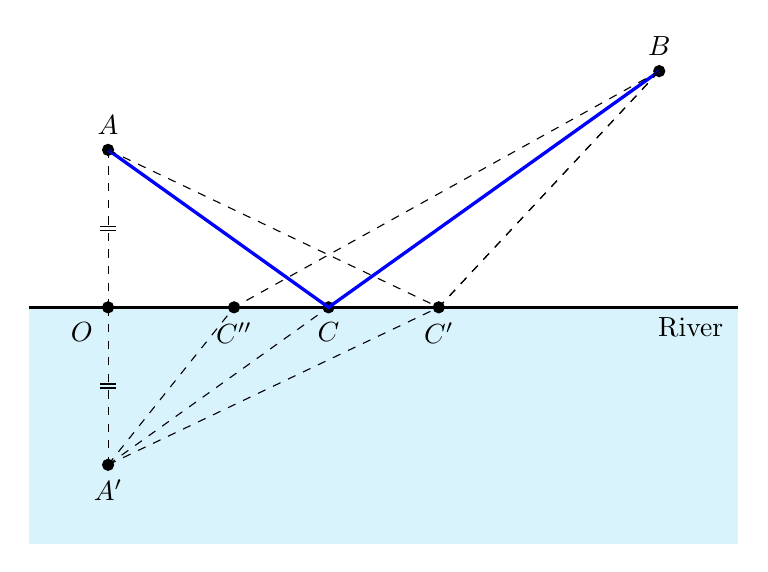
\begin{tikzpicture}
  %% Heron's problem

  % Params
  \def\xA{1}
  \def\yA{2}
  \def\xB{8}
  \def\yB{3}
  \def\xCp{5.2}
  \def\xCpp{2.6}

  % River y=0
  \fill[cyan!15] (\xA-1,0) rectangle (\xB+1,-\yA-1);
  \draw[very thick] (\xA-1,0) -- (\xB+1,0);
  \node at (\xB+0.4,0) [below] {River};

  % Coords
  \coordinate (A) at (\xA,\yA);
  \coordinate (B) at (\xB,\yB);
  \coordinate (O) at (\xA,0);  % Projection of A onto river
  \coordinate (Aprime) at (\xA,{-\yA});  % Reflection of A over river
  \coordinate (Cprime) at (\xCp,0);
  \coordinate (Cdoubleprime) at (\xCpp,0);

  % Paths
  \path[name path=lineAB] (Aprime) -- (B);
  \path[name path=river] (\xA-1,0) -- (\xB+1,0);
  \path[name intersections={of=lineAB and river, by=C}];

  % Points
  \draw[fill=black] (A) circle (2pt);
  \draw[fill=black] (B) circle (2pt);
  \draw[fill=black] (O) circle (2pt);
  \draw[fill=black] (Aprime) circle (2pt);
  \draw[fill=black] (C) circle (2pt);
  \draw[fill=black] (Cprime) circle (2pt);
  \draw[fill=black] (Cdoubleprime) circle (2pt);

  % Labels
  \node[above=2pt] at (A) {\( A \)};
  \node[above=2pt] at (B) {\( B \)};
  \node[below left=2pt] at (O) {\( O \)};
  \node[below=2pt] at (Aprime) {\( A' \)};
  \node[below=2pt] at (C) {\( C \)};
  \node[below=2pt] at (Cprime) {\( C' \)};
  \node[below=2pt] at (Cdoubleprime) {\( C'' \)};

  % Segments
  \draw[dashed] (A) -- (O);
  \draw[dashed] (O) -- (Aprime);
  \draw[dashed] (Aprime) -- (B);
  \draw[very thick, blue] (A) -- (C) -- (B);
  \draw[dashed] (Aprime) -- (Cprime) -- (B);
  \draw[dashed] (A) -- (Cprime) -- (B);
  \draw[dashed] (Aprime) -- (Cdoubleprime) -- (B);

  % Segment ticks
  \draw[line width=0.5pt] (\xA-0.1,0.975) -- (\xA+0.1,0.975);
  \draw[line width=0.5pt] (\xA-0.1,1.025) -- (\xA+0.1,1.025);
  \draw[line width=0.5pt] (\xA-0.1,-0.975) -- (\xA+0.1,-0.975);
  \draw[line width=0.5pt] (\xA-0.1,-1.025) -- (\xA+0.1,-1.025);

\end{tikzpicture}
\end{document}
